\section{Resultados}

Se muestra a continuación los resultados numéricos obtenidos. En la Figuras \ref{fig_1} y \ref{fig_2} se muestra el campo de velocidad y de presión de la mitad inferior de la tubería.  En la Figura \ref{fig_3} se comparar los resultados de perfil de velocidad en $x=Lx/2$ para modificando la razón de proporción de los volúmenes. En la medida que se vuelven menos regulares (alejandose de la relación 1:1, $Lx=5$, $nx=50$, $Ly=1$, $ny=10$) los resultados se alejan de la solución analítica. \\

En la Tabla \ref{resultados_1} se determinan los número CFL que aseguran la estabilidad. Notar CFL disminuye en la medida que Re disminuye.

\begin{table}[H]
\centering
\begin{tabular}{|l|lll|} \hline
Re & 2000	& 1500	& 1000 \\
CFL & 0.30	& 0.23	& 0.15 \\
T[s] & 18.908	& 45.036 & 19.840 \\ \hline
\end{tabular}
\caption{Número CFL que asegura la convergencia para cada Re ($Lx=5$, $Ly=1$, $Nx=50$, $Ny=10$)} \label{resultados_1}
\end{table}


\begin{figure}[H]
\centering
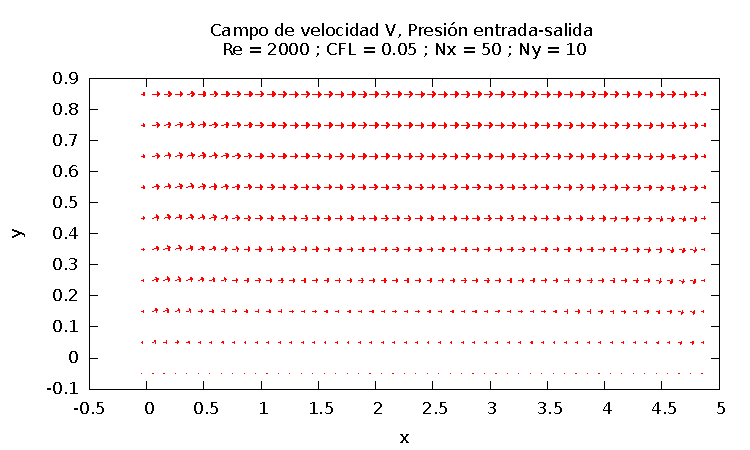
\includegraphics[width=1\textwidth]{./fig1_1/fig1_1/velocity_field.pdf}
\caption{} \label{fig_1}
\end{figure}

\begin{figure} [H]
\centering
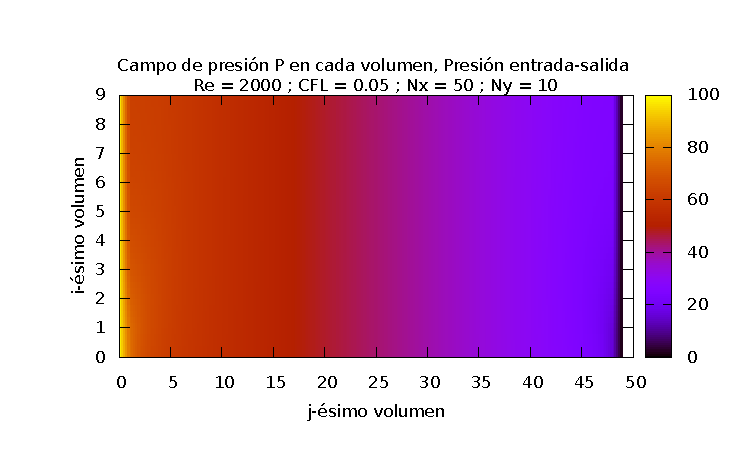
\includegraphics[width=1\textwidth]{./fig1_1/fig1_1/pressure_field.pdf}
\caption{} \label{fig_2}
\end{figure}

\begin{figure} [H]
\centering
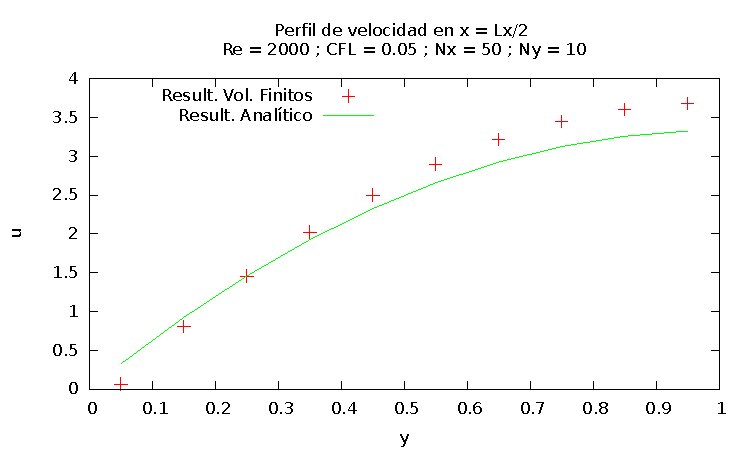
\includegraphics[width=0.8\textwidth]{./fig1_1/fig1_1/velocity_profile.pdf}
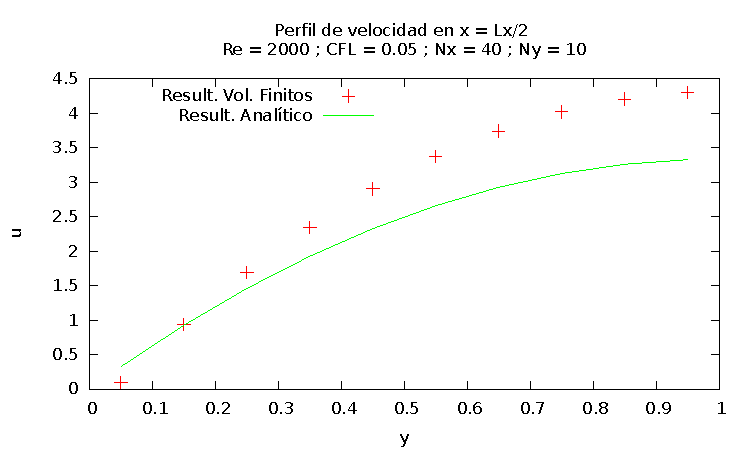
\includegraphics[width=0.8\textwidth]{./fig1_1/fig1_2/velocity_profile.pdf}
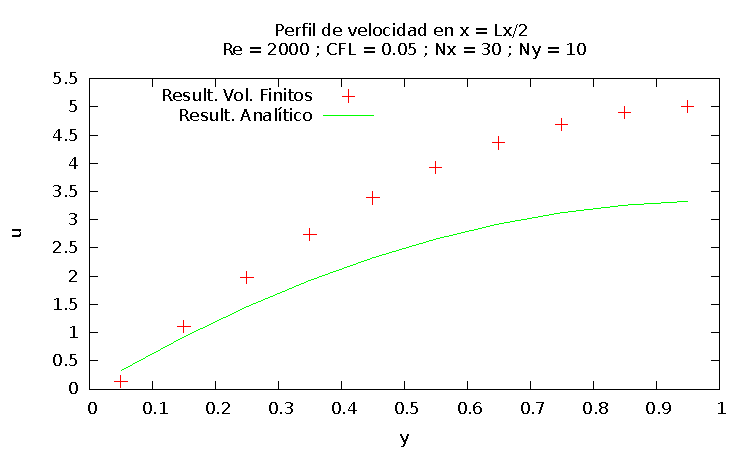
\includegraphics[width=0.8\textwidth]{./fig1_1/fig1_3/velocity_profile.pdf}
\caption{} \label{fig_3}
\end{figure}
